\documentclass[11pt,a4paper]{article}
\usepackage[margin=2.2cm]{geometry}
\usepackage{amsmath,amssymb,graphicx,booktabs}
\usepackage[T1]{fontenc}
\setlength{\parindent}{0pt}
\setlength{\parskip}{6pt}
\setlength{\emergencystretch}{2em}
\newcommand{\code}[1]{\texttt{#1}}
\begin{document}
\begin{center}
{\Large\bfseries Assignment 1: MicroGrad}\\[5pt]
{\large Scalar Autograd Engine}\\[8pt]
Ahmed Hossam Abdallah -- 23P0109\\
CSE485-CSE488: Deep Learning\\
Ain Shams University, Faculty of Engineering
\end{center}

\section{Scalar graph and local derivatives}
The implementation has two parts: a scalar automatic differentiation engine
in \code{engine.py} and a small neural network API in \code{nn.py}. The engine
uses only Python's standard library. No PyTorch operations are used.

Each \code{Value} stores its scalar \code{data}, its accumulated \code{grad},
the input nodes in \code{\_prev}, an operation name and an optional label.
The operation also installs a \code{\_backward} closure. This closure knows
the local derivative and adds its contribution to the input gradients.
For an operation $z=f(a,b)$ inside a loss $L$, the chain rule gives
\[
\frac{\partial L}{\partial a}\mathrel{+}=
\frac{\partial L}{\partial z}\frac{\partial z}{\partial a}.
\]
The same rule is applied to $b$. Constants are converted to \code{Value}
objects so mixed expressions such as \code{2 + x} build the same kind of graph.

\begin{center}
\begin{tabular}{lll}
\toprule
Operation & Local derivative(s) & Gradient contribution to $a$\\
\midrule
$z=a+b$ & $z_a=1,\ z_b=1$ & $\bar z$\\
$z=ab$ & $z_a=b,\ z_b=a$ & $b\bar z$\\
$z=a^p$ & $z_a=pa^{p-1}$ & $pa^{p-1}\bar z$\\
$z=\exp(a)$ & $z_a=\exp(a)=z$ & $z\bar z$\\
$z=\tanh(a)$ & $z_a=1-z^2$ & $(1-z^2)\bar z$\\
\bottomrule
\end{tabular}
\end{center}
Here $\bar z=\partial L/\partial z$. For the power operation, $p$ is a Python
integer or float, not a differentiable exponent. When $p=0$, the derivative
is zero; the backward closure skips the power calculation to avoid evaluating
$0^{-1}$ at $a=0$. Python evaluates the forward expression $0^0$ as $1$.

The tanh derivative follows directly from the quotient rule:
\[
t=\frac{e^a-e^{-a}}{e^a+e^{-a}},\qquad
t'=\frac{(e^a+e^{-a})^2-(e^a-e^{-a})^2}
{(e^a+e^{-a})^2}=1-t^2.
\]
The implementation uses \code{math.tanh} for the forward result, avoiding
overflow from manually forming large exponentials. Negation, subtraction
and division reuse multiplication, addition and powers:
$-a=(-1)a$, $a-b=a+(-b)$ and $a/b=ab^{-1}$.
Consequently, $\partial(a/b)/\partial a=1/b$ and
$\partial(a/b)/\partial b=-a/b^2$ for $b\ne0$.

\newpage
\section{Topological order and backpropagation}
The graph is directed from inputs to outputs. A local backward closure must
run only after all downstream operations have contributed to its output
gradient. The implementation follows the assignment's depth-first search:
\begin{verbatim}
topo = []
visited = set()

def build_topo(node):
    if node not in visited:
        visited.add(node)
        for child in node._prev:
            build_topo(child)
        topo.append(node)

build_topo(self)
\end{verbatim}
Appending after visiting the inputs creates a post-order list: each input
appears before the operation that consumes it. \code{backward()} seeds the
output gradient with $1$ because $\partial L/\partial L=1$, then calls
\code{\_backward()} on the reversed list. This puts every operation before
its inputs during backpropagation. DFS costs $O(V+E)$ time and $O(V)$ extra
space for a graph with $V$ nodes and $E$ dependency links.

\subsection{Why gradients must accumulate}
Consider the shared-node example from the assignment:
\[
a=3,\qquad c=a+a=6,\qquad d=ca=18.
\]
One possible DFS order is $[a,c,d]$, and the backward order is $[d,c,a]$.
Starting from $\bar d=1$, multiplication gives
\[
\bar c\mathrel{+}=a\bar d=3,\qquad
\bar a\mathrel{+}=c\bar d=6.
\]
Then $c=a+a$ contributes $\bar c$ twice to $a$:
\[
\bar a=6+3+3=12.
\]
This agrees with $d=2a^2$, whose derivative at $a=3$ is $4a=12$.
Assigning gradients with \code{=} would lose earlier contributions.

\subsection{The two ordering traps}
\textbf{Appending before visiting inputs:} reversing a pre-order list can
process an input before its full downstream gradient is available. A
chain-rule computation would then propagate an incomplete value.

\textbf{Omitting the visited set:} a shared subgraph could appear more than
once in the topological list, causing its backward closure to propagate
the same accumulated gradient repeatedly. A valid computational DAG does
not itself create an infinite loop; the relevant issue here is repeated
visits and double-counting. The visited set ensures one execution per node.
Even though \code{\_prev} is a set and stores $a$ once in $a+a$, the addition
closure still adds both operand contributions. Traversal and differentiation
therefore preserve the correct behavior for repeated operands.

\newpage
\section{Neural network API and training design}
\subsection{Neuron, Layer and MLP}
A neuron with $n$ inputs evaluates
\[
s=\sum_{j=1}^{n}w_jx_j+b,\qquad y=\tanh(s).
\]
Each weight and the bias is a separate \code{Value}, initialized uniformly
on $[-1,1]$ as requested in the template. Random initialization breaks the
symmetry between neurons. The local gradients are
\[
\frac{\partial y}{\partial w_j}=(1-y^2)x_j,\qquad
\frac{\partial y}{\partial b}=1-y^2,\qquad
\frac{\partial y}{\partial x_j}=(1-y^2)w_j.
\]
These derivatives are obtained by composing the existing scalar operations;
the neuron needs no separate backward implementation.

A \code{Layer} calls its neurons on the same input. It returns a scalar
\code{Value} when it has one neuron, and a list otherwise, following the
template. An \code{MLP} sends each layer's output to the next layer. If an
intermediate layer returns one scalar, the MLP wraps it in a list before
passing it onward. A neuron also checks the input length so \code{zip}
cannot silently ignore missing or extra inputs.

\code{parameters()} returns references to the existing weights and biases,
flattened across neurons and layers. It does not make copies. For a
$2\to4\to1$ network, the count is
\[
(2+1)\cdot4+(4+1)\cdot1=17.
\]
\code{zero\_grad()} calls \code{reset\_grad()} on every parameter. This matters
because the engine deliberately adds gradient contributions.

\subsection{Dataset and reproducibility}
The assignment does not specify a dataset. The demo therefore uses a small,
included noisy XOR CSV. Its four centers are $(\pm1,\pm1)$, with independent
Gaussian noise of standard deviation $0.2$ on each coordinate. Targets are
$-1$ for equal center signs and $+1$ otherwise, matching the tanh range.
The data generator uses seed $23$ and rounds coordinates to six decimals.
There are $12$ training and $6$ test points per cluster: $48$ training and
$24$ held-out test points. Both sets are balanced. No downloads are needed.

The demo compares a single neuron with the 17-parameter MLP. Each model uses
initialization seed $7$, learning rate $0.1$ and $600$ full-batch updates.
The settings are fixed, and the test rows are used only for evaluation.
The loss and update are
\[
L=\frac1N\sum_i(\hat y_i-y_i)^2,\qquad
\frac{\partial L}{\partial\hat y_i}=\frac2N(\hat y_i-y_i),\qquad
p\leftarrow p-0.1\frac{\partial L}{\partial p}.
\]
Each step builds a fresh loss graph, clears parameter gradients, runs
backpropagation and updates parameter data. Tanh is also used at the output
to follow the assignment API. Class predictions use threshold zero.

\newpage
\section{Measured results}
The following values come from executing \code{demo.ipynb} from a clean
kernel. The JSON results and full loss histories are included in
\code{results/}. Accuracy uses the sign of the tanh output.

\begin{center}
\begin{tabular}{lrrrrr}
\toprule
Model & Params & Train MSE & Test MSE & Train acc. & Test acc.\\
\midrule
Single neuron & 3 & 1.013736 & 1.013165 & 75\% & 75\%\\
MLP ($2$-$4$-$1$) & 17 & 0.004055 & 0.003387 & 100\% & 100\%\\
\bottomrule
\end{tabular}
\end{center}
The MLP training MSE decreases from $1.363100$ to $0.004055$. Its predictions
on the exact four XOR points, in order $(-1,-1),(-1,1),(1,-1),(1,1)$, are
$-0.94974$, $0.96804$, $0.95820$ and $-0.95212$. All four signs are correct.

\begin{center}
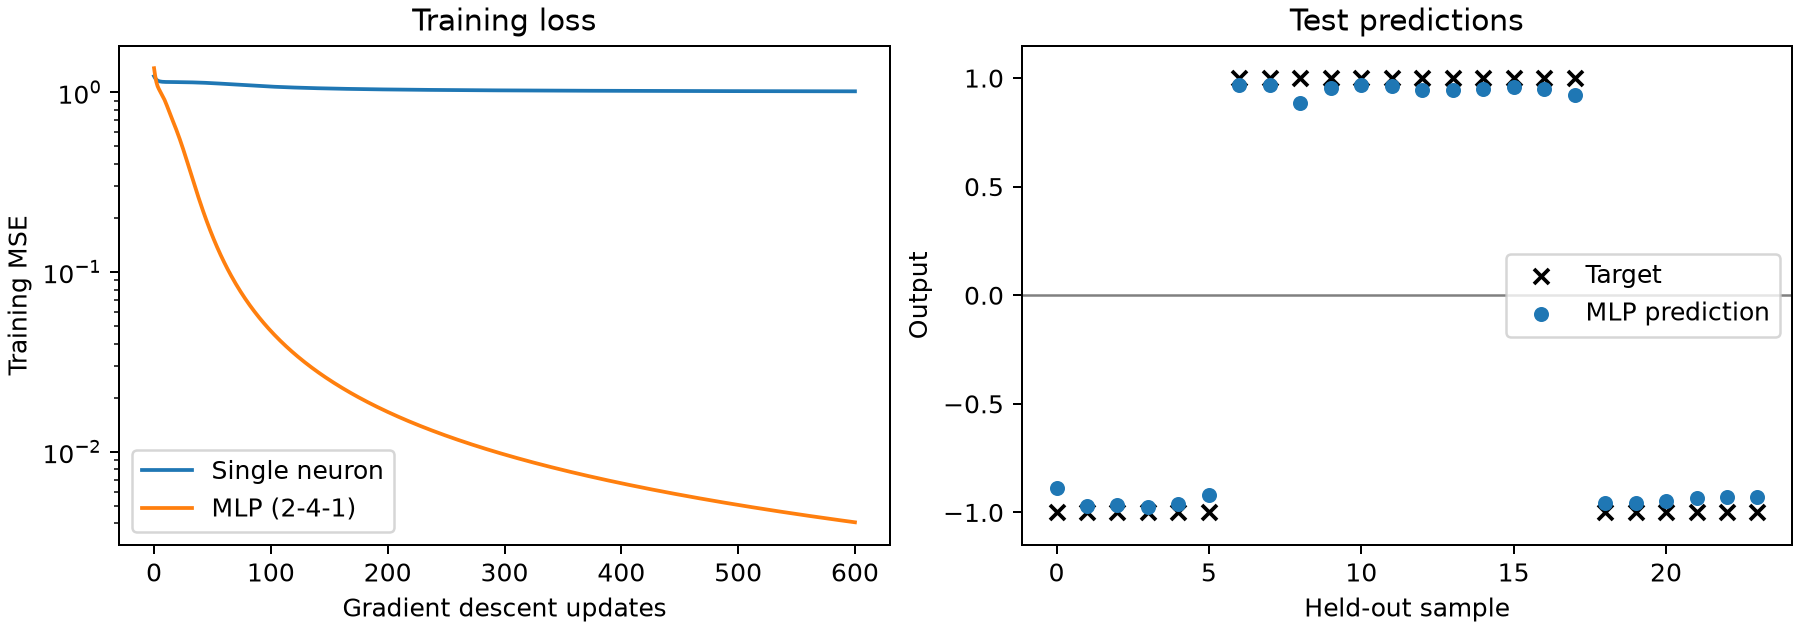
\includegraphics[width=\linewidth]{../figures/training_results.png}
\end{center}
{\small\textbf{Figure 1.} Training loss over 600 updates, and MLP outputs for
the 24 held-out samples. The vertical loss scale is logarithmic.}

\begin{center}
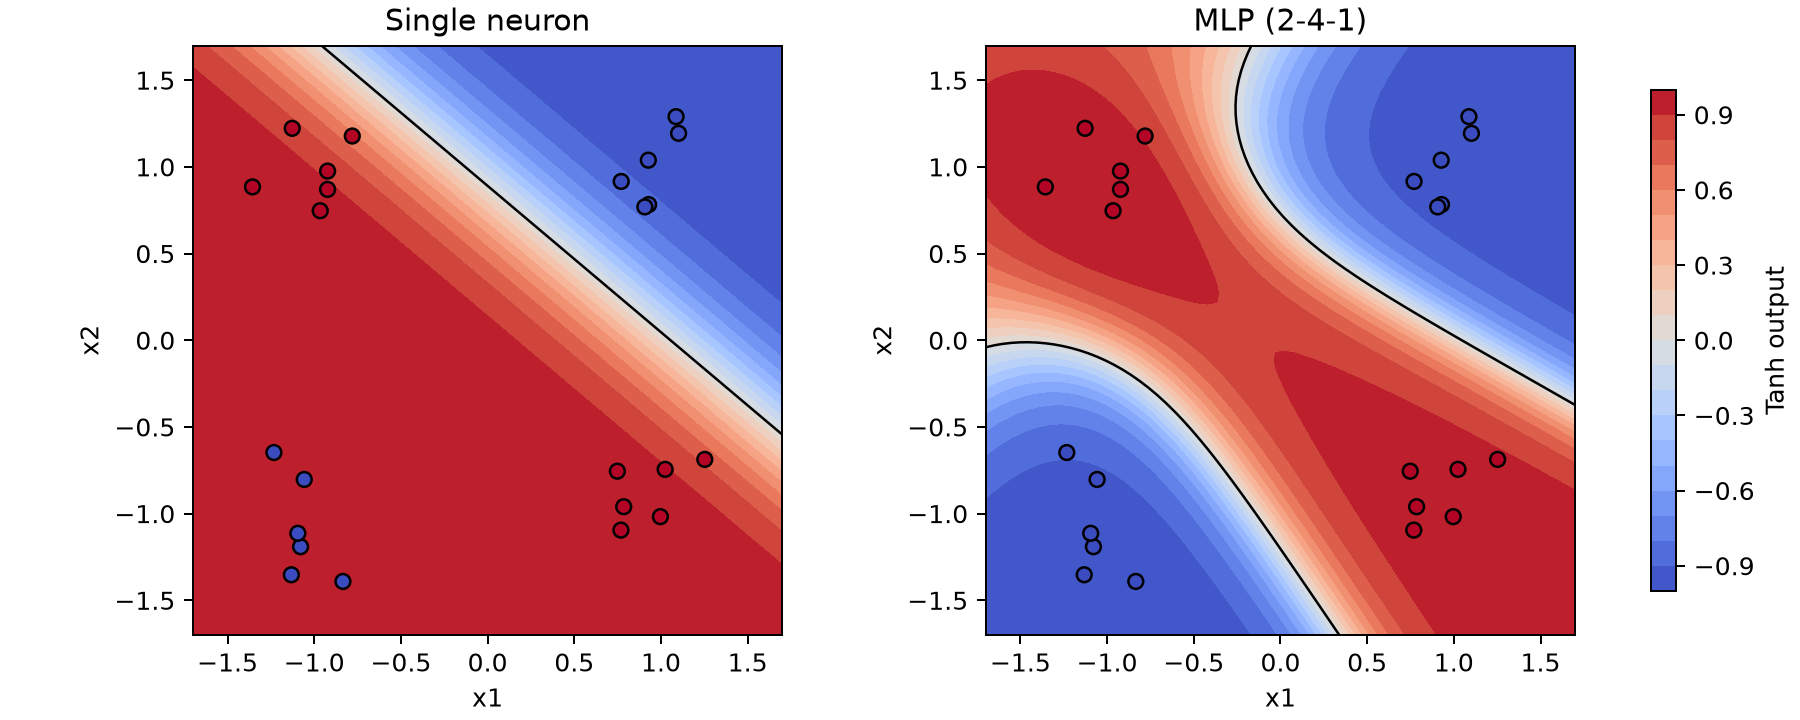
\includegraphics[width=\linewidth]{../figures/decision_boundary.png}
\end{center}
{\small\textbf{Figure 2.} Learned outputs over the input plane. Markers are
held-out samples colored by target; the black contour is output zero.}

One neuron has the zero-output boundary $w_1x_1+w_2x_2+b=0$, which is a
straight line. It cannot separate all four alternating XOR regions. Hidden
tanh neurons create nonlinear features, allowing the MLP to represent the
required separation. The result shows this on the sampled clusters; it is
not a guarantee about every point in the plane.

\newpage
\section{Verification and limitations}
\subsection{Gradient checks and tests}
For numerical checking, each parameter $p$ is perturbed separately:
\[
g_{\rm FD}=\frac{f(p+h)-f(p-h)}{2h},\qquad h=10^{-6}.
\]
The original parameter is restored after both evaluations. The notebook
checks all 17 parameters of a separate $2\to4\to1$ MLP with initialization
seed $11$ and input $(0.3,-0.8)$. The largest absolute difference from
backpropagation is $2.459\times10^{-11}$, below the $10^{-6}$ tolerance.
This is a local numerical check, not a proof for every possible input.

The 12 original instructor tests pass locally. They check scalar operations,
types, activations, the chain rule, the shared-node graph, division by zero,
and the network API. Eleven additional test cases also pass, giving 23 local
passes in total. The added checks cover numerical scalar and network
derivatives, zero powers, post-order traversal, a known neuron output,
clearing nonzero gradients in all three modules, one-neuron hidden layers,
incorrect input lengths and decreasing training loss. The original tests
and grading workflow have not been edited.

The additional tests do not increase the course autograder's score total.
Its workflow copies only \code{src/engine.py} and \code{src/nn.py} from the
submission and runs the instructor tests. A local pass must still be
confirmed by the actual PR grader.

\subsection{Conceptual points and practical limits}
\textbf{Why reverse-mode differentiation?} One backward traversal computes
gradients for all parameters of a scalar loss. Finite differences would
need two forward evaluations per parameter and introduce a step-size error.

\textbf{Why clear gradients between updates?} Without clearing them, the
new derivative would be added to previous updates' derivatives. That would
change the gradient descent update. Intentional gradient accumulation is
possible, but it is not used in this demo.

\textbf{Can the same graph be reused?} The current backward pass accumulates
gradients in intermediate nodes too. Repeating backward on the same graph
requires clearing those intermediates as well as the parameters. The demo
builds a new graph every step, so clearing model parameters is sufficient.

\textbf{What limits the implementation?} Every scalar operation allocates
Python objects; there is no tensor batching or GPU execution. Deep graphs
can exceed the recursive DFS stack limit. Very large exponentials can
overflow, and tanh saturation makes derivatives small. The engine assumes
ordinary real-valued differentiable inputs; division by zero remains an
error and variable exponents are not supported.

The experiment uses only one training seed and 24 test samples drawn from a
simple synthetic distribution. Its 100\% test accuracy demonstrates this
pipeline on this split, not performance on a realistic dataset.

\subsection*{Assignment sources and deliverables}
The implementation requirements and traversal algorithm follow the supplied
\emph{Assignment 1: MicroGrad (Scalar Autograd Engine)} PDF and course
template README. The LMS archive includes the code, executed notebook,
dataset, results, figures, this compiled PDF and its LaTeX source.
The separate GitHub submission uses branch
\code{Ahmed-Hossam-Abdallah\_23P0109}.
\end{document}
